\chapter{Method}
The method chapter gives a high level overview of the method used in this work. More detailed steps are delegated to the results (Chapter \ref{cha:Results}) which contains implementation details and the evaluation of the implementation.

The problem is clearly defined from the previous chapters, especially Section \ref{sec:TheProblem} which goes into detail with examples. Alternatives for this implementation are then explored and presented to the project manager of the Spade compiler -- which also happens to be the supervisor for this work -- for evaluation and consideration. This allows a flexible approach to implementation where the goal is to find the best implementation. This way of working is a take on the agile methodologies.

After a viable solution is picked, it is time to implement that solution. Since the project is open source special care should be taken to make the changes easily accessible and available after this work is written. A list of the repositories and versions of each software are available in the Appendix \ref{app:VersionsAndGitHashes} and the \hyperfootnote{git-repository for this work}{https://github.com/FredTheDino/thesis-spade-lang}. Steps of the implementation and details relevant to the results are discussed in the implementation details sections in Chapter \ref{cha:Results}. A full evaluation for each of the potential implementations and details about these implementations that are deemed relevant and interesting are mentioned in Chapter \ref{cha:Results}. For full details it is probably best to read the source code. 

The implementation is then evaluated using some simple expressions, a FIR-filter \hyperfootnote{available at the thesis website}{https://github.com/FredTheDino/thesis-spade-lang/tree/main/messing/fir} and spade-memory-display. The modified version of spade-memory-display is available \hyperfootnote{in a forked repository}{https://github.com/FredTheDino/spade-memory-display-wli-fork}. The programs will also be evaluated by a place and route, this work uses nextpnr version \verb+0.6-29-g54b20457+ for all the PNR done in this work. All the statistics from the PNR step is then saved, and all the experiments are run at least 50 times to give some credibility to the results. The most interesting metric is the number of LUTs used in the final design since the LUTs would show where the designs could remove unnecessary complexity springing from the more complex input to functions -- LUTs is a very good proxy measure for the complexity of the circuit.

\section{Finding Implementations and Creative Problem Solving}

\begin{center}
\begin{figure}[h!]
\centering
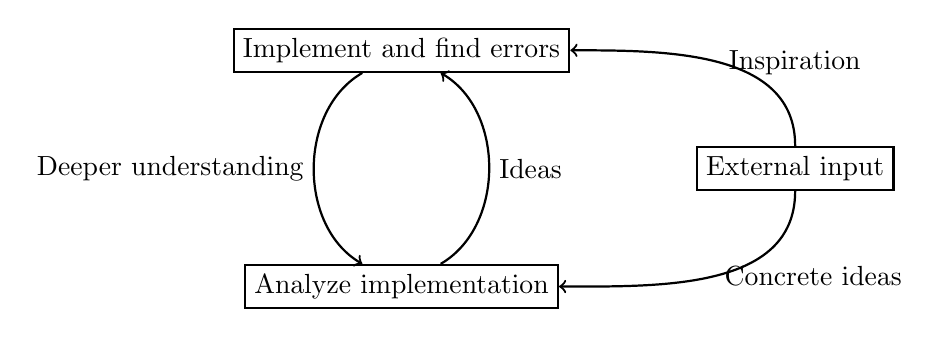
\begin{tikzpicture}[thick, node/.style = {draw}]
  \node[node] (a) at (0,0) {Analyze implementation};
  \node[node] (b) at (0,3) {Implement and find errors};
  \node[node] (c) at (5,1.5) {External input};

  \draw[->, align=left] (a) to[out=30,in=-30] node[right]{Ideas} (b);
  \draw[->, align=left] (b) to[out=-150,in=150] node[left]{Deeper understanding} (a);
  \draw[->] (c) to[out=-90,in=0] node[right]{Concrete ideas} (a);
  \draw[->] (c) to[out=90,in=0] node[right]{Inspiration} (b);
\end{tikzpicture}
\caption{The creative process of solving complex problems according to the author.}
\label{figCreativeProcess}
\end{figure}
\end{center}

Solving complex problems is a creative process. Programmings languages are required to be complex since the ideas expressed in them are themselves complex. Complex problems require complex tools. The complexity requires that the programming language
has a certain degree of quality -- else the programming language quickly becomes useless and frustrating to use. To find a solution of sufficient quality requires trial and error and a good dose of analysis. Understanding partial solutions to a complex problem is a natural way of finding a solution that is higher in quality and hopefully good enough for the programming language to be usable. Figure \ref{figCreativeProcess} contains a visualization of how these steps integrate with each other.

% NOTE[fs]: Quite an abrupt end to the section, consider a few sentences about what is to follow
% NOTE[et]: No...
